\documentclass{ximera}

%\usepackage{todonotes}

\newcommand{\todo}{}

\usepackage{tkz-euclide}
\tikzset{>=stealth} %% cool arrow head
\tikzset{shorten <>/.style={ shorten >=#1, shorten <=#1 } } %% allows shorter vectors

\usetikzlibrary{backgrounds} %% for boxes around graphs
\usetikzlibrary{shapes,positioning}  %% Clouds and stars
\usetikzlibrary{matrix} %% for matrix
\usepgfplotslibrary{polar} %% for polar plots
\usetkzobj{all}
\usepackage[makeroom]{cancel} %% for strike outs
%\usepackage{mathtools} %% for pretty underbrace % Breaks Ximera
\usepackage{multicol}





\usepackage{array}
\setlength{\extrarowheight}{+.1cm}   
\newdimen\digitwidth
\settowidth\digitwidth{9}
\def\divrule#1#2{
\noalign{\moveright#1\digitwidth
\vbox{\hrule width#2\digitwidth}}}





\newcommand{\RR}{\mathbb R}
\newcommand{\R}{\mathbb R}
\newcommand{\N}{\mathbb N}
\newcommand{\Z}{\mathbb Z}

%\renewcommand{\d}{\,d\!}
\renewcommand{\d}{\mathop{}\!d}
\newcommand{\dd}[2][]{\frac{\d #1}{\d #2}}
\renewcommand{\l}{\ell}
\newcommand{\ddx}{\frac{d}{\d x}}

\newcommand{\zeroOverZero}{\ensuremath{\boldsymbol{\tfrac{0}{0}}}}
\newcommand{\inftyOverInfty}{\ensuremath{\boldsymbol{\tfrac{\infty}{\infty}}}}
\newcommand{\zeroOverInfty}{\ensuremath{\boldsymbol{\tfrac{0}{\infty}}}}
\newcommand{\zeroTimesInfty}{\ensuremath{\small\boldsymbol{0\cdot \infty}}}
\newcommand{\inftyMinusInfty}{\ensuremath{\small\boldsymbol{\infty - \infty}}}
\newcommand{\oneToInfty}{\ensuremath{\boldsymbol{1^\infty}}}
\newcommand{\zeroToZero}{\ensuremath{\boldsymbol{0^0}}}
\newcommand{\inftyToZero}{\ensuremath{\boldsymbol{\infty^0}}}


\newcommand{\numOverZero}{\ensuremath{\boldsymbol{\tfrac{\#}{0}}}}
\newcommand{\dfn}{\textbf}
%\newcommand{\unit}{\,\mathrm}
\newcommand{\unit}{\mathop{}\!\mathrm}
\newcommand{\eval}[1]{\bigg[ #1 \bigg]}
\newcommand{\seq}[1]{\left( #1 \right)}
\renewcommand{\epsilon}{\varepsilon}
\renewcommand{\iff}{\Leftrightarrow}

\DeclareMathOperator{\arccot}{arccot}
\DeclareMathOperator{\arcsec}{arcsec}
\DeclareMathOperator{\arccsc}{arccsc}
\DeclareMathOperator{\si}{Si}

\newcommand{\tightoverset}[2]{%
  \mathop{#2}\limits^{\vbox to -.5ex{\kern-0.75ex\hbox{$#1$}\vss}}}
\newcommand{\arrowvec}[1]{\tightoverset{\scriptstyle\rightharpoonup}{#1}}
\renewcommand{\vec}{\mathbf}


\colorlet{textColor}{black} 
\colorlet{background}{white}
\colorlet{penColor}{blue!50!black} % Color of a curve in a plot
\colorlet{penColor2}{red!50!black}% Color of a curve in a plot
\colorlet{penColor3}{red!50!blue} % Color of a curve in a plot
\colorlet{penColor4}{green!50!black} % Color of a curve in a plot
\colorlet{penColor5}{orange!80!black} % Color of a curve in a plot
\colorlet{fill1}{penColor!20} % Color of fill in a plot
\colorlet{fill2}{penColor2!20} % Color of fill in a plot
\colorlet{fillp}{fill1} % Color of positive area
\colorlet{filln}{penColor2!20} % Color of negative area
\colorlet{fill3}{penColor3!20} % Fill
\colorlet{fill4}{penColor4!20} % Fill
\colorlet{fill5}{penColor5!20} % Fill
\colorlet{gridColor}{gray!50} % Color of grid in a plot

\newcommand{\surfaceColor}{violet}
\newcommand{\surfaceColorTwo}{redyellow}
\newcommand{\sliceColor}{greenyellow}




\pgfmathdeclarefunction{gauss}{2}{% gives gaussian
  \pgfmathparse{1/(#2*sqrt(2*pi))*exp(-((x-#1)^2)/(2*#2^2))}%
}


%%%%%%%%%%%%%
%% Vectors
%%%%%%%%%%%%%

%% Simple horiz vectors
\renewcommand{\vector}[1]{\left\langle #1\right\rangle}


%% %% Complex Horiz Vectors with angle brackets
%% \makeatletter
%% \renewcommand{\vector}[2][ , ]{\left\langle%
%%   \def\nextitem{\def\nextitem{#1}}%
%%   \@for \el:=#2\do{\nextitem\el}\right\rangle%
%% }
%% \makeatother

%% %% Vertical Vectors
%% \def\vector#1{\begin{bmatrix}\vecListA#1,,\end{bmatrix}}
%% \def\vecListA#1,{\if,#1,\else #1\cr \expandafter \vecListA \fi}

%%%%%%%%%%%%%
%% End of vectors
%%%%%%%%%%%%%

%\newcommand{\fullwidth}{}
%\newcommand{\normalwidth}{}



%% makes a snazzy t-chart for evaluating functions
%\newenvironment{tchart}{\rowcolors{2}{}{background!90!textColor}\array}{\endarray}

%%This is to help with formatting on future title pages.
\newenvironment{sectionOutcomes}{}{} 



%% Flowchart stuff
%\tikzstyle{startstop} = [rectangle, rounded corners, minimum width=3cm, minimum height=1cm,text centered, draw=black]
%\tikzstyle{question} = [rectangle, minimum width=3cm, minimum height=1cm, text centered, draw=black]
%\tikzstyle{decision} = [trapezium, trapezium left angle=70, trapezium right angle=110, minimum width=3cm, minimum height=1cm, text centered, draw=black]
%\tikzstyle{question} = [rectangle, rounded corners, minimum width=3cm, minimum height=1cm,text centered, draw=black]
%\tikzstyle{process} = [rectangle, minimum width=3cm, minimum height=1cm, text centered, draw=black]
%\tikzstyle{decision} = [trapezium, trapezium left angle=70, trapezium right angle=110, minimum width=3cm, minimum height=1cm, text centered, draw=black]

\definecolor{myblue}{rgb}{0,0,0.8}
\definecolor{myred}{rgb}{0.8,0,0}


\outcome{Define a cross product.}
\outcome{Compute cross products.}
\outcome{Use cross products in applied settings.}

\title[Dig-In:]{Cross Product}

\begin{document}
\begin{abstract}
  The cross product is a special way to multiply two vectors in $\mathbb{R}^3$
\end{abstract}
\maketitle

There is no ``nice'' way to ``multiply'' two vectors and obtain another vector in general.

However, in the special case of $\mathbb{R}^3$, there is an important multiplication operation called ``the cross product''.  

The cross product is linked inextricably to the determinant, so we will first review the determinant before introducing this new operation.

\section{Determinants}

\begin{definition}
	The determinant on $\mathbb{R}^3$ is a function $\textrm{Det}$ which takes three vectors $\vec{a},\vec{b},\vec{c} \in \mathbb{R}^3$ as input and returns a number as its output.
	
	It is given by the formula
	
	\[
	\textrm{Det}\left(\begin{bmatrix} a_1 \\ a_2 \\a_3 \end{bmatrix}, \begin{bmatrix} b_1 \\ b_2 \\b_3 \end{bmatrix}, \begin{bmatrix} c_1 \\ c_2 \\c_3 \end{bmatrix} \right)  = a_1b_2c_3+b_1c_2a_3+c_1a_2b_3-a_3b_2c_1-b_3c_2a_1-c_3a_2b_1
	\]
	
	\end{definition}
	
	Often, instead of writing the three vectors as distinct entries, we write them as columns in a matrix:
	
	\[
	\textrm{Det}\left(\begin{bmatrix} a_1 \\ a_2 \\a_3 \end{bmatrix}, \begin{bmatrix} b_1 \\ b_2 \\b_3 \end{bmatrix}, \begin{bmatrix} c_1 \\ c_2 \\c_3 \end{bmatrix} \right) = 
	\begin{vmatrix} 
	a_1 & b_1 & c_1\\
	a_2 & b_2 & c_2\\
	a_3 & b_3 & c_3\\
	\end{vmatrix}
	\]
	
	
	We can remember this formula by writing the first two columns of the matrix to the right of the matrix, and using the following pattern:
	
%Credit for the following image goes to http://tex.stackexchange.com/a/257063
	\begin{image}
\begin{tikzpicture}[
strip/.style = {
    draw=#1,%color
    line width=1em, opacity=0.2,
    shorten <=-2mm,shorten >=-2mm,
                            },
                    ]
\matrix (mtrx)  [matrix of math nodes,
                 column sep=1em,
                 nodes={text height=1ex,text width=2ex}]
{
|[red]|+
    & |[red]|+
          & \color{red}+\color{blue}-
                & |[blue]|-
                      & |[blue]|-   \\[3.3mm,between origins]
a_1 & b_1 & c_1 & a_1 & a_2         \\
a_2 & b_2 & c_2 & a_2 & b_2         \\
a_3 & b_3 & c_3 & a_3 & b_3         \\
};
\draw[thick] (mtrx-2-1.north) -| (mtrx-4-1.south west)
                              -- (mtrx-4-1.south);
\draw[thick] (mtrx-2-3.north) -| (mtrx-4-3.south east)
                              -- (mtrx-4-3.south);
\path[draw,strip=blue]
    (mtrx-4-1.center) edge (mtrx-2-3.center)
    (mtrx-4-2.center) edge (mtrx-2-4.center)
    (mtrx-4-3.center)  --  (mtrx-2-5.center);
\path[draw,strip=red]
    (mtrx-2-1.center) edge (mtrx-4-3.center)
    (mtrx-2-2.center) edge (mtrx-4-4.center)
    (mtrx-2-3.center)  --  (mtrx-4-5.center);
\end{tikzpicture}
	\end{image}
	
	\begin{question}
		\[
	\begin{vmatrix} 
	1 & 4 & 7\\
	2 & 5 & 8\\
	3 & 6 & 9\\
	\end{vmatrix}
	= \answer{0}
		\]
		
		\begin{hint}
			\begin{align*}
			1(5)(9)+4(8)(3)+7(2)(6) - 3(5)(7) - 6(8)(1)-9(2)(4) &= 45+96+84-105-48-72\\
			&=225-225\\
			&=0
			\end{align*}
		\end{hint}
	\end{question}
	
	\begin{question}
		If $\textrm{Det}(\vec{a},\vec{b},\vec{c}) = 12$, what is $\textrm{Det}(\vec{b},\vec{a},\vec{c})$?
		
		\[
		\textrm{Det}(\vec{b},\vec{a},\vec{c}) = \answer{-12}
		\]
		
		\begin{hint}
	\[\begin{vmatrix} 
	b_1 & a_1 & c_1\\
	b_2 & a_2 & c_2\\
	b_3 & a_3 & c_3\\
	\end{vmatrix}
	=b_1a_2c_3+a_2c_3b_3+c_1b_2a_3-b_3a_2c_1-a_3c_3b_1-c_3b_2a_1
	\]
	
	But this (make sure you check!) equal to $-\textrm{Det}(\vec{a},\vec{b},\vec{c})$.  Thus the answer is $-12$.
		\end{hint}
	\end{question}
	
	\begin{question}
		\[
		\textrm{Det}(\vec{a},\vec{a},\vec{b}) = \answer{0}
		\]
		
		\begin{hint}
			If you write out the definition, you will see that all the terms cancel, and you get $0$
		\end{hint}
	\end{question}
	
	\begin{question}
		Assume $\textrm{Det}(\vec{a},\vec{b},\vec{c}) = 3$.  Then 
		
		\[
		\textrm{Det}(5\vec{a},\vec{b},2\vec{c}) = \answer{30}
		\]
		
		\begin{hint}
			Since each term has an entry from $\vec{a},\vec{b}$ and $\vec{c}$, and each entry of each vector is getting multiplied by the same constant, we get an extra factor of $10$ in each term.  Thus the answer is $30$.
		\end{hint}
	\end{question}
	
	\begin{question}
		Assume $\textrm{Det}(\vec{a},\vec{b},\vec{c}) = 3$ and $\textrm{Det}(\vec{a},\vec{b},\vec{d}) = 4$.
		
		\[
		\textrm{Det}(\vec{a},\vec{b},\vec{c}+\vec{d}) = \answer{7}
		\]
		
		\begin{hint}
			Writing out the definition, and distributing, you will see that this is equal to the sum of the two original determinants.  So the answer is $7$.
		\end{hint}
	\end{question}
	
	The last few exercises strongly suggest the following theorem (which you have essentially already proven by doing the exercises above):
	
	\begin{theorem}
		The determinant enjoys the following properties, and is in fact the \textbf{only} function enjoying such properties:
		
		\begin{itemize}
			\item Alternating:  Switching any pair of entries in the determinant switches the sign.  For example $\textrm{Det}(\vec{a},\vec{b},\vec{c}) = -\textrm{Det}(\vec{c},\vec{b},\vec{a})$.
			\item Factor out scalars:  Multiplying any entry by a constant scales the determinant by that constant.  For example
			 $\textrm{Det}(k\vec{a},\vec{b},\vec{c}) = k\textrm{Det}(\vec{a},\vec{b},\vec{c}) $
			 
			 \item Respect addition:  For example $\textrm{Det}(\vec{a},\vec{b}+\vec{d},\vec{c}) = \textrm{Det}(\vec{a},\vec{b},\vec{c}) +\textrm{Det}(\vec{a},\vec{d},\vec{c}) $ 
			 
			 \item $\textrm{Det}(\vec{i},\vec{j},\vec{k}) = 1 $
			 \end{itemize}
	\end{theorem}
	
	\begin{observation}
		By the alternating property, if the same vector appears more than once as an argument in a determinant, then the determinant must be zero.
		
		For example consider $\textrm{Det}(\vec{a},\vec{a},\vec{b})$. By the alternating property we must have
		
		\[
		\textrm{Det}(\vec{a},\vec{a},\vec{b}) = -\textrm{Det}(\vec{a},\vec{a},\vec{b})
		\]
		
		but this implies 
		
		\[
		\textrm{Det}(\vec{a},\vec{a},\vec{b})=0
		\]
	\end{observation}
	
	We will not prove that the determinant is the only function with these properties, but that is an important point.  If you ever wondered where this crazy formula came from, this explains it.  If you want these $4$ nice looking properties, there is only one function which does it and it is this one.  You should be able to prove that yourself, using just the properties.  Just start with a general $\textrm{Det}(\vec{a},\vec{b},\vec{c}) $, and use the properties to reduce it to sums of determinants involving only $\vec{i},\vec{j}$ and $\vec{k}$.  The formula for the determinant will pop out.  
	
	It turns out that the determinant has the following geometric interpretation:
	
	\begin{theorem}
		If $\vec{a},\vec{b},\vec{c} \in \mathbb{R}^3$, then they span a parallelepiped. The volume of this parallelepiped is $\left|\textrm{Det}(\vec{a},\vec{b},\vec{c})\right|$. If this parallelepiped is not degenerate (has nonzero volume), then the sign of $\textrm{Det}(\vec{a},\vec{b},\vec{c})$ tells you whether the trio of vectors is \dfn{positively oriented} or \dfn{negatively oriented} (this is the definition of positively and negatively oriented).
	\end{theorem} 
	
	\begin{question}
		Let $\vec{a} = \vector{1,1,1}$, $\vec{b} = \vector{1,0,1}$ and $\vec{c} = \vector{1,0,0}$.
		
		Is $(\vec{a},\vec{b},\vec{c})$ positively or negatively oriented?
		
		\begin{multipleChoice}
			\choice[correct]{positively}
			\choice{negatively}
		\end{multipleChoice}
		
		What is the volume of the parallelepiped spanned by these three vectors?
		
		\[
		\textrm{Volume} = \answer{1}
		\]
		
		\begin{hint}
			\begin{align*}
				\begin{vmatrix}
					1 & 1 & 1\\
					1 & 0 & 0\\
					1 & 1 & 0
				\end{vmatrix} &=
				1(0)(0)+1(0)(1)+1(1)(1)-1(0)(1)-1(1)(1)-0(1)(1)\\
				&=1
			\end{align*}
			
			Thus this trio is positively oriented, and its volume is $1$.
		\end{hint}
	\end{question}
	
	\begin{question}
		Do the vectors $\vector{1,2,2}$, $\vector{3,4,1}$ and $\vector{5,8,5}$ all lie in the same plane?
		
		\begin{multipleChoice}
			\choice{No}
			\choice[correct]{Yes}
		\end{multipleChoice}
		
		\begin{hint}
			They will lie in the same plane iff the parallelepiped they span is degenerate, aka its volume is $0$.
		\end{hint}
		
		\begin{hint}
			So we just need to see whether the determinant of these three vectors is zero or not.
		\end{hint}
		
		\begin{hint}
			\begin{align*}
				\begin{vmatrix}
				1&3&5\\
				2&4&8\\
				2&1&5
				\end{vmatrix} &= 1(4)(5)+3(8)(2)+5(2)(1)-2(4)(5)-1(8)(1)-5(2)(3)\\
					&=20+48+10-40-8-30\\
					&=78-78\\
					&=0
			\end{align*}
			
			Thus the vectors must all lie in the same plane.  In fact, we can see that $2\vector{1,2,2}+\vector{3,4,1}=\vector{5,8,5}$, which confirms this fact.
		\end{hint}
		
 	\end{question}
	

	
	We will not explicitly prove this theorem here.  However, you should be able to convince yourself that the oriented volume function $\textrm{Vol}(\vec{a},\vec{b},\vec{c})$ satisfies all $4$ conditions of the determinant above.  Since there is only one function satisfying these properties, the volume function must be given by the determinant.
	
	Here is a nice geometric interpretation of orientation.
	
	\begin{theorem}
	Consider the trio of vectors $(\vec{a},\vec{b},\vec{c})$.  Assume that they form a nondegenerate parallelepiped.  Then the vectors $\vec{a}$ and $\vec{b}$ define a plane.  There are two sides to this plane.  If you take your right hand, and curl your fingers from $\vec{a}$ to $\vec{b}$, your thumb will be pointing to one side of the plane.  If $\vec{c}$ is on this side, then the trio is positively oriented.  Otherwise it is negatively oriented.
		\begin{center}
		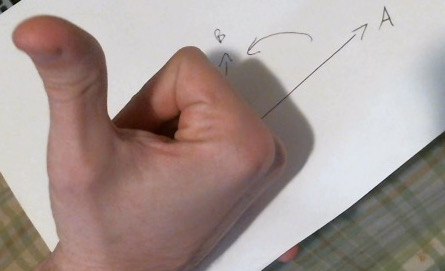
\includegraphics[width=3 in]{RHR.jpg}
		
		 All vectors on the same side of the plane that the thumb is pointing are positively oriented with respect to $(A,B)$
		\end{center}
	\end{theorem}
	

\section{Cross Products}

\begin{definition}
	The cross product of two vectors is given by the formula
	
	\[
		\vector{a_1,a_2,a_3} \times \vector{b_1,b_2,b_3} = \vector{a_2b_3-a_3b_2, -(a_1b_3-a_3b_1), a_1b_2-a_2b_1}
	\]
\end{definition}		

\begin{question}
	\[
	\vector{2,3,1} \times \vector{1,1,1} = \vector{\answer{2},\answer{-1},\answer{-1}}
	\]
	
	\begin{hint}
		\begin{align*}
			\vector{2,3,1} \times \vector{1,1,1} &= \vector{3(1)-1(1),-(2(1)-1(1)), 2(1)-3(1)}\\
				&=\vector{2,-1,-1}
		\end{align*}
	\end{hint}
\end{question}

This formula is pretty horrible, and you may be wondering why anyone would ever care about such a thing.  The answer is that is has a very nice relationship to the determinate, and hence to volumes, areas, and orientations:

\begin{theorem}[Triple product theorem]
If $\vec{a},\vec{b},$ and $\vec{c}$ are vectors in $\mathbb{R}^3$, then 

\[
(\vec{a} \times \vec{b}) \cdot \vec{c} = \textrm{Det}(\vec{a},\vec{b},\vec{c}) 
\]
\end{theorem}

\begin{proof}

The proof is just a computation:

\begin{align*}
	(\vec{a} \times \vec{b}) \cdot \vec{c} &= \vector{a_2b_3-a_3b_2, -(a_1b_3-a_3b_1), a_1b_2-a_2b_1} \cdot \vector{c_1,c_2,c_3}\\
	&=c_1a_2b_3-c_1a_3b_2+c_2a_3b_1-c_2a_1b_3+c_3a_1b_2-c_3a_2b_1\\
	&=\textrm{Det}(\vec{a},\vec{b},\vec{c}) 
\end{align*}
\end{proof}

This theorem will allow us to gain massive insight into the geometric nature of the cross product:

\begin{theorem}
	$\vec{a} \times \vec{b}$ is perpendicular to both $\vec{a}$ and $\vec{b}$.
\end{theorem}

\begin{proof}
	We need to show that $(\vec{a} \times \vec{b}) \cdot \vec{a} = 0 $ and $\vec{a} \times \vec{b} \cdot \vec{b} = 0$.  Let's just do the first one:
	
	\[
	(\vec{a} \times \vec{b}) \cdot \vec{a} = \textrm{Det}(\vec{a},\vec{b},\vec{a})
	\]
	
	But this must be zero by the alternating property.
	
	The other case follows similarly.
\end{proof}

\begin{theorem}
	The length of $\vec{a} \times \vec{b}$ is the area of the parallelogram spanned by $\vec{a}$ and $\vec{b}$.  Also the trio $(\vec{a},\vec{b},\vec{a} \times \vec{b})$ is positively oriented.
\end{theorem}

\begin{proof}
	\begin{align*}
	|\vec{a} \times \vec{b}|^2  &=(\vec{a} \times \vec{b}) \cdot (\vec{a} \times \vec{b})\\
		&=\textrm{Det}(\vec{a},\vec{b},\vec{a} \times \vec{b})
	\end{align*}
	
	Note that this already shows that the trio is positively oriented, since the determinant $\textrm{Det}(\vec{a},\vec{b},\vec{a} \times \vec{b})$ is equal to the square of a length, which must be positive.
	
	Also note that $\textrm{Det}(\vec{a},\vec{b},\vec{a} \times \vec{b})$ represents the volume of the parallelepiped spanned by $\vec{a}$, $\vec{b}$, and $\vec{a} \times \vec{b}$.  Since we already know that $vec{a} \times \vec{b}$ is perpendicular to the plane spanned by $\vec{a}$ and $\vec{b}$, then just by geometry (base times height) we know that this volume is equal to $A |vec{a} \times \vec{b}|$, where $A$ is the area of the parallelogram spanned by $\vec{a}$ and $\vec{b}$.  Hence
	
	\[
	|\vec{a} \times \vec{b}|^2 = A |\vec{a} \times \vec{b}|
	\]
	
	From which the claim follows.
\end{proof}

\begin{question}
	What is the area of the parallelogram spanned by $\vector{1,2,4}$ and $\vector{2,3,1}$?
	
	\[
	\textrm{Area} = \answer{\sqrt{150}}
	\]
	
	\begin{hint}
		\[
		\vector{1,2,4} \times \vector{2,3,1} = \vector{-10,7,-1}
		\]
	\end{hint}
	
	
	\begin{hint}
		\begin{align*}
			\left| \vector{-10,7,-1} \right| &= \sqrt{ \vector{-10,7,-1} \cdot  \vector{-10,7,-1}}\\
				&=\sqrt{100+49+1}\\
				&=\sqrt{150}
		\end{align*}
		
		Since the area of the parallelogram is the length of the cross product, we are done.
	\end{hint}
\end{question}

Putting all of these ideas together we have:

\begin{theorem}
	$\vec{a} \times \vec{b}$ is the vector perpendicular to the plane spanned by $\vec{a}$ and $\vec{b}$ which points in the ``positive direction'', as given by the right hand rule, and whose length is the area of the parallelogram spanned by $\vec{a}$ and $\vec{b}$.  
\end{theorem}

\begin{observation}
Since the height of this parallelogram is $|\vec{b}| \sin\theta$ and its length is $|\vec{a}|$ where $\theta$ is the angle between $\vec{a}$ and $\vec{b}$, we could also say that $|\vec{a} \times \vec{b}| = |\vec{a}||vec{b}| \sin\theta$
\end{observation}

\begin{question}
	Using the geometric ideas above, compute the following cross products.  It may be helpful to use  your left hand to form a coordinate system (where your index finger is the positive $z$ axis, your thumb is the positive $x$ axis, and your middle finger is the positive $y$ axis), and use your right hand to determine orientation.
	
	\begin{align*}
		\vector{1,0,0} \times \vector{0,1,0} = \vector{\answer{0},\answer{0},\answer{1}}\\
		\vector{0,1,0} \times \vector{1,0,0} = \vector{\answer{0},\answer{0},\answer{-1}}\\
		\vector{0,0,1} \times \vector{0,1,0} = \vector{\answer{-1},\answer{0},\answer{0}}\\
		\vector{0,1,0} \times \vector{0,1,0} = \vector{\answer{0},\answer{0},\answer{0}}\\
	\end{align*}
\end{question}

Below, we summarize some rules for working with cross products:

\begin{theorem}

Let $\vec{v},\vec{w},\vec{u} \in \mathbb{R}^3$.  Then

	\begin{itemize}
		\item $\vec{v} \times \vec{w}  = -\vec{w} \times \vec{v}$ (Anti-commutivity property )
		\item $(\vec{v}+\vec{w}) \times \vec{u} = \vec{v} \times \vec{u}+\vec{w} \times \vec{u}$ (Right distributive property)
		\item $\vec{u} \times (\vec{v} +\vec{w}) = \vec{u} \times \vec{v}+\vec{u}\times\vec{w}$ (Left distributive property)
		\item $a\vec{v} \times b\vec{w} = ab \vec{v} \times \vec{w}$ (Respects scalar multiplication)
		\item $\vec{v} \times \vec{v} = 0$
		\item $\vec{i} \times \vec{j} = \vec{k}$
		\item $\vec{i} \times \vec{k} = \vec{-j}$
		\item $\vec{j} \times \vec{k} = \vec{i}$
	\end{itemize}
	
	Moreover, these properties determine the cross product uniquely.
\end{theorem}

\begin{question}
	Using only these rules, compute $(3\vec{i}+k) \times (2\vec{j}+\vec{i})$
	\[
	(3\vec{i}+\vec{k}) \times (2\vec{j}+\vec{i}) = \answer{-2}\vec{i}+\answer{1}\vec{j}+\answer{6}\vec{k}
	\]
	
	\begin{hint}
		\begin{align*}
		(3\vec{i}+\vec{k}) \times (2\vec{j}+\vec{i}) &= (3\vec{i}+\vec{k}) \times 2\vec{j}+(3\vec{i}+\vec{k}) \times\vec{i}\\
			&=3\vec{i} \times 2\vec{j}+\vec{k}\times 2\vec{j}+3\vec{i} \times \vec{i} +\vec{k} \times \vec{i}\\
			&=6 \vec{i} \times \vec{j}+2 \vec{k} \times \vec{j}+3\vec{i} \times \vec{i} +\vec{k} \times \vec{i}\\
			&=6 \vec{i} \times \vec{j}+-2 \vec{j} \times \vec{k}+3\vec{i} \times \vec{i} -\vec{i} \times \vec{k}\\
			&=6 \vec{k}+-2 \vec{i}+3\vec{0} -(-\vec{j})\\
			&=-2\vec{i}+1\vec{j}+6\vec{k}
		\end{align*}
	\end{hint}
\end{question}



\section{Applications}

In addition to the geometric applications we have already seen (calculating the area of parallelograms), we can also use the cross product in some physical applications.

\subsection{Torque}

Imagine turning a wrench.  The wrench originates at a point $O$ and terminates at a point $P$.  Let $\vec{r} = \overrightarrow{OP}$.  You apply a force $\vec{F}$ to the end of the wrench.  If $\vec{F}$ points in the same direction as $\vec{r}$, the bolt will not twist at all, since you will just be pulling on the handle.  If $\vec{F}$ is perpendicular to the handle, then we expect quite a bit of twisting to occur.

\begin{definition}
	The torque $\vec{\tau}$ obtained by applying a force $\vec{F}$ to a lever arm with position vector $\vec{r}$ is given by
	
	\[
	\vec{\tau} = \vec{r} \times \vec{F} 
	\]
\end{definition}

\begin{question}
	A pipe of length $3 \unit{m}$  has a force of magnitude $2 \unit{N}$ applied to it as shown below:
	
	\begin{image}
  \begin{tikzpicture}
	\begin{axis}[
            xmin=-1,xmax=5,ymin=-1,ymax=3,
            clip=false,
            axis lines=center,
            ticks=none,
            unit vector ratio*=1 1 1,
            xlabel=$x$, ylabel=$y$,
            %ytick={-2,-1,...,7},
	    %xtick={-2,-1,...,10},
	   % grid = major,
            every axis y label/.style={at=(current axis.above origin),anchor=south},
            every axis x label/.style={at=(current axis.right of origin),anchor=west},
          ]
          \addplot[very thick,penColor,->] plot coordinates {(0,0) (1,2)};
          \addplot[very thick,penColor2,->] plot coordinates {(1,2) (0.5,3)};
          \addplot[very thick,penColor, dashed] plot coordinates {(1,2) (2,4)};
          \node at (axis cs:1, 2.6) [textColor] {$\frac{\pi}{3}$};
           \node at (axis cs:0.6, 0.7) [penColor] {$\vec{r}$};
           \node at (axis cs:0.6, 2.4) [penColor2] {$\vec{F}$};
        \end{axis}
        
\end{tikzpicture}

\end{image}

Assuming the $z$ -axis is coming towards you (out of the page), is the torque produced in the positive or negative $z$ direction?

\begin{multipleChoice}
	\choice[correct]{Positive}
	\choice{Negative}
\end{multipleChoice}

\[
|\vec{tau}| = \answer{3\sqrt{3}}
\]

\begin{hint}
	Using the right hand rule, we see that the vector points in the positive $z$ direction.
\end{hint}

\begin{hint}
The angle between the two vectors is $\frac{\pi}{3}$, so the area of the area of the parallelogram spanned by these vectors is $2(3)\sin(\frac{\pi}{3}) = 3\sqrt{3}$
\end{hint}

\end{question}

\subsection{Magnetism} 

When a charged particle moves through a magnetic field, it experiences a force.  If the charge is $q$, the velocity of the particle is $\vec{v}$, and the magnetic field is $\vec{B}$, then the force is given by

\[
\vec{F} = q\vec{v} \times \vec{B}
\]

\begin{question}
	A particle with negative charge $-2$ enters a constant magnetic field given by $\vec{B} = \vec{i}+2\vec{j}$.  The velocity vector of the particle is  $\vec{v} = \vec{k}+\vec{i}$.  What is the force acting on the particle?
	
	\[
	\vec{F} = \answer{4}\vec{i}+\answer{-2}\vec{j}+\answer{-2}\vec{k}
	\]
	
	\begin{hint}
		\begin{align*}
			\vec{F} &= q\vec{v} \times \vec{B}\\
				&= -2 ( \vec{k}+\vec{i}) \times (\vec{i}+2\vec{j})\\
				&=-2( \vec{k} \times \vec{i}+2\vec{k} \times \vec{j}+\vec{i} \times \vec{i}+\vec{i} \times \vec{j})\\
				&=-2(\vec{j}-2\vec{i}+\vec{0}+\vec{k})\\
				&=4\vec{i}-2\vec{j}-2\vec{k}
		\end{align*}
	\end{hint}
\end{question}

	
\end{document}
